\chapter{Mô hình hóa hành vi}

\section{Sơ đồ trình tự}

\subsection{Xử lý sự cố (nhánh thuê ngoài)}

\begin{figure}[h]
\centering
\IfFileExists{figures/sequence-incident.png}{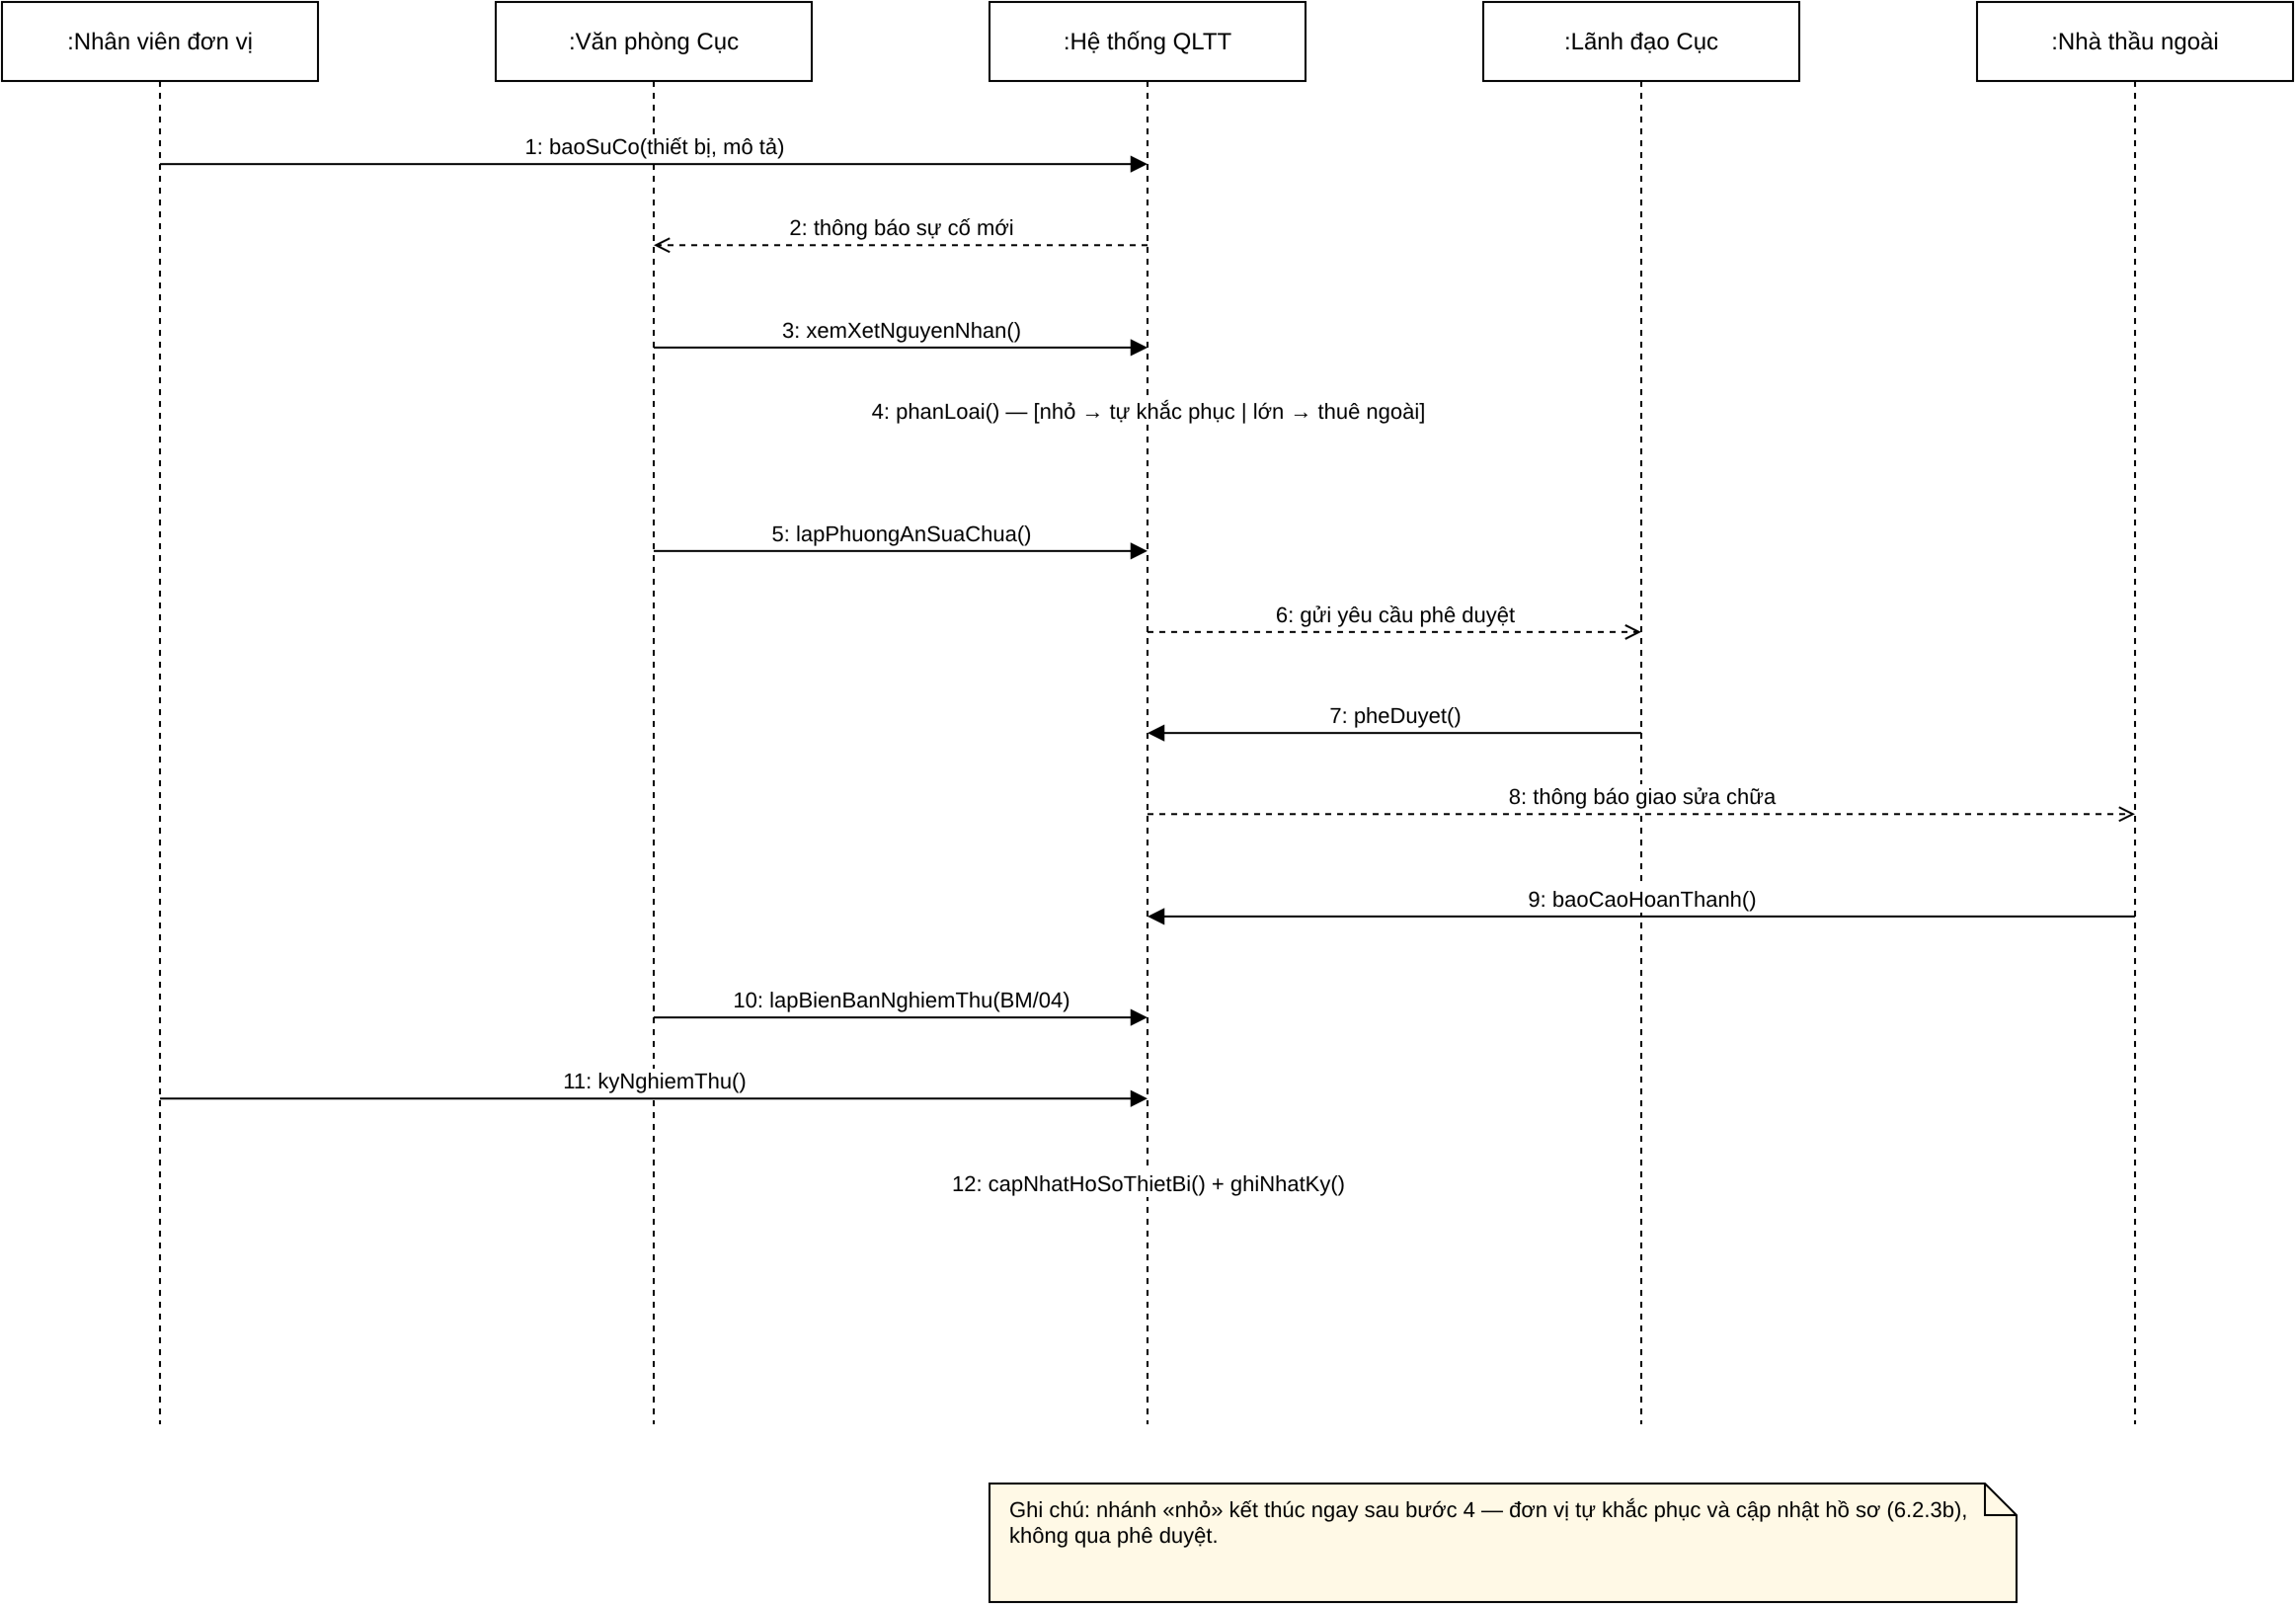
\includegraphics[width=0.94\textwidth]{figures/sequence-incident.png}}{\fbox{\parbox{0.9\textwidth}{\centering Sơ đồ trình tự xử lý sự cố (file \texttt{docs/diagrams/04-sequence.drawio}, trang 1)}}}
\caption{Sơ đồ trình tự — xử lý sự cố thuê ngoài}
\label{fig:seq-incident}
\end{figure}

Diễn giải Hình~\ref{fig:seq-incident}:
\begin{enumerate}
  \item Đơn vị gửi \texttt{baoSuCo(thiết bị, mô tả)}; hệ thống sinh mã sự cố, chuyển thiết bị sang ``Sự cố'' và thông báo cho Văn phòng Cục.
  \item Văn phòng Cục gọi \texttt{xemXetNguyenNhan()}; hệ thống \texttt{phanLoai()}: nếu nhỏ $\rightarrow$ kết thúc ngay (đơn vị tự khắc phục, không qua duyệt); nếu lớn $\rightarrow$ tiếp tục.
  \item Văn phòng Cục \texttt{lapPhuongAnSuaChua()}; hệ thống gửi yêu cầu phê duyệt tới Lãnh đạo Cục.
  \item Lãnh đạo Cục \texttt{pheDuyet()}; hệ thống thông báo giao sửa chữa cho nhà thầu, thiết bị chuyển ``Đang sửa chữa''.
  \item Nhà thầu \texttt{baoCaoHoanThanh()}; Văn phòng Cục \texttt{lapBienBanNghiemThu(BM/04)}; các bên \texttt{kyNghiemThu()}.
  \item Khi đủ chữ ký, hệ thống tự thực hiện \texttt{capNhatHoSoThietBi() + ghiNhatKy()} — đóng sự cố, trả thiết bị về ``Hoạt động''.
\end{enumerate}

\subsection{Lập và phê duyệt kế hoạch bảo dưỡng}

\begin{figure}[h]
\centering
\IfFileExists{figures/sequence-plan.png}{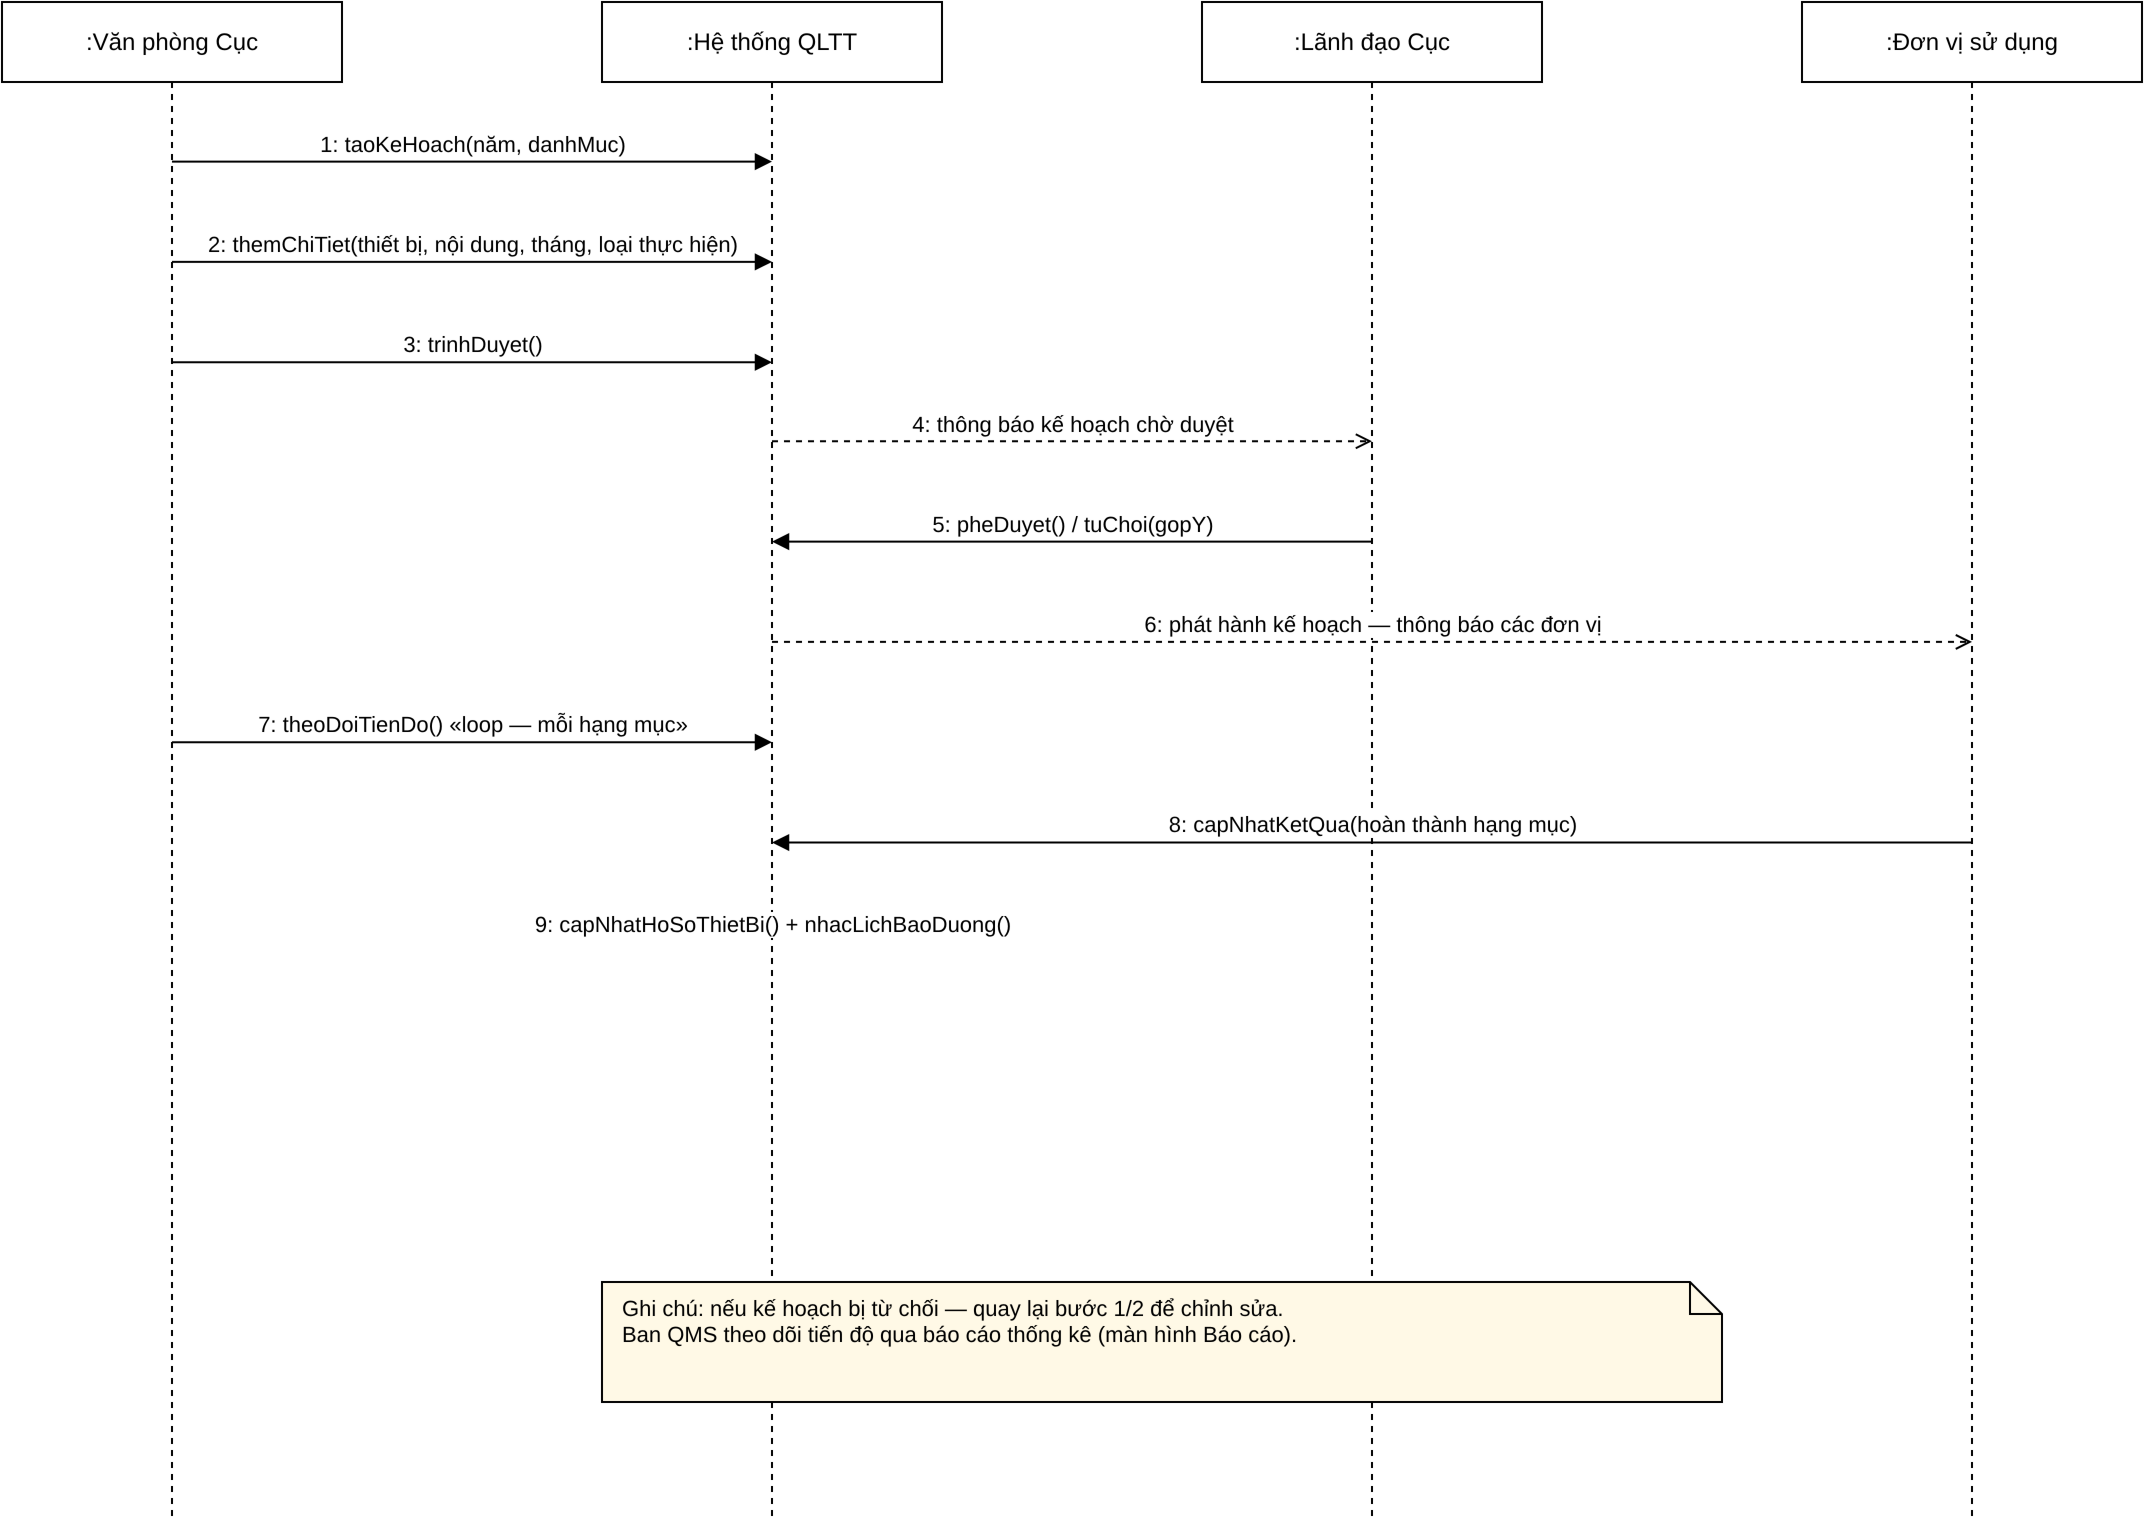
\includegraphics[width=0.9\textwidth]{figures/sequence-plan.png}}{\fbox{\parbox{0.9\textwidth}{\centering Sơ đồ trình tự kế hoạch bảo dưỡng (file \texttt{docs/diagrams/04-sequence.drawio}, trang 2)}}}
\caption{Sơ đồ trình tự — lập và phê duyệt kế hoạch hàng năm}
\label{fig:seq-plan}
\end{figure}

Diễn giải Hình~\ref{fig:seq-plan}: Văn phòng Cục \texttt{taoKeHoach(năm)} rồi \texttt{themChiTiet(...)} cho từng hạng mục (bước 1--2); \texttt{trinhDuyet()} (bước 3) đưa kế hoạch sang ``Chờ duyệt'' và thông báo Lãnh đạo Cục (bước 4). Lãnh đạo Cục \texttt{pheDuyet()/tuChoi(gopY)} (bước 5) — nếu bị từ chối thì quay lại bước 1--2 chỉnh sửa. Khi được duyệt, hệ thống phát hành kế hoạch tới các đơn vị (bước 6); vòng lặp theo dõi tiến độ (bước 7--8) kết thúc bằng \texttt{capNhatHoSoThietBi() + nhacLichBaoDuong()} (bước 9). Ban QMS theo dõi tiến độ qua màn hình báo cáo.

\section{Sơ đồ trạng thái}

\subsection{Vòng đời TrangThietBi}

\begin{figure}[h]
\centering
\IfFileExists{figures/state-equipment.png}{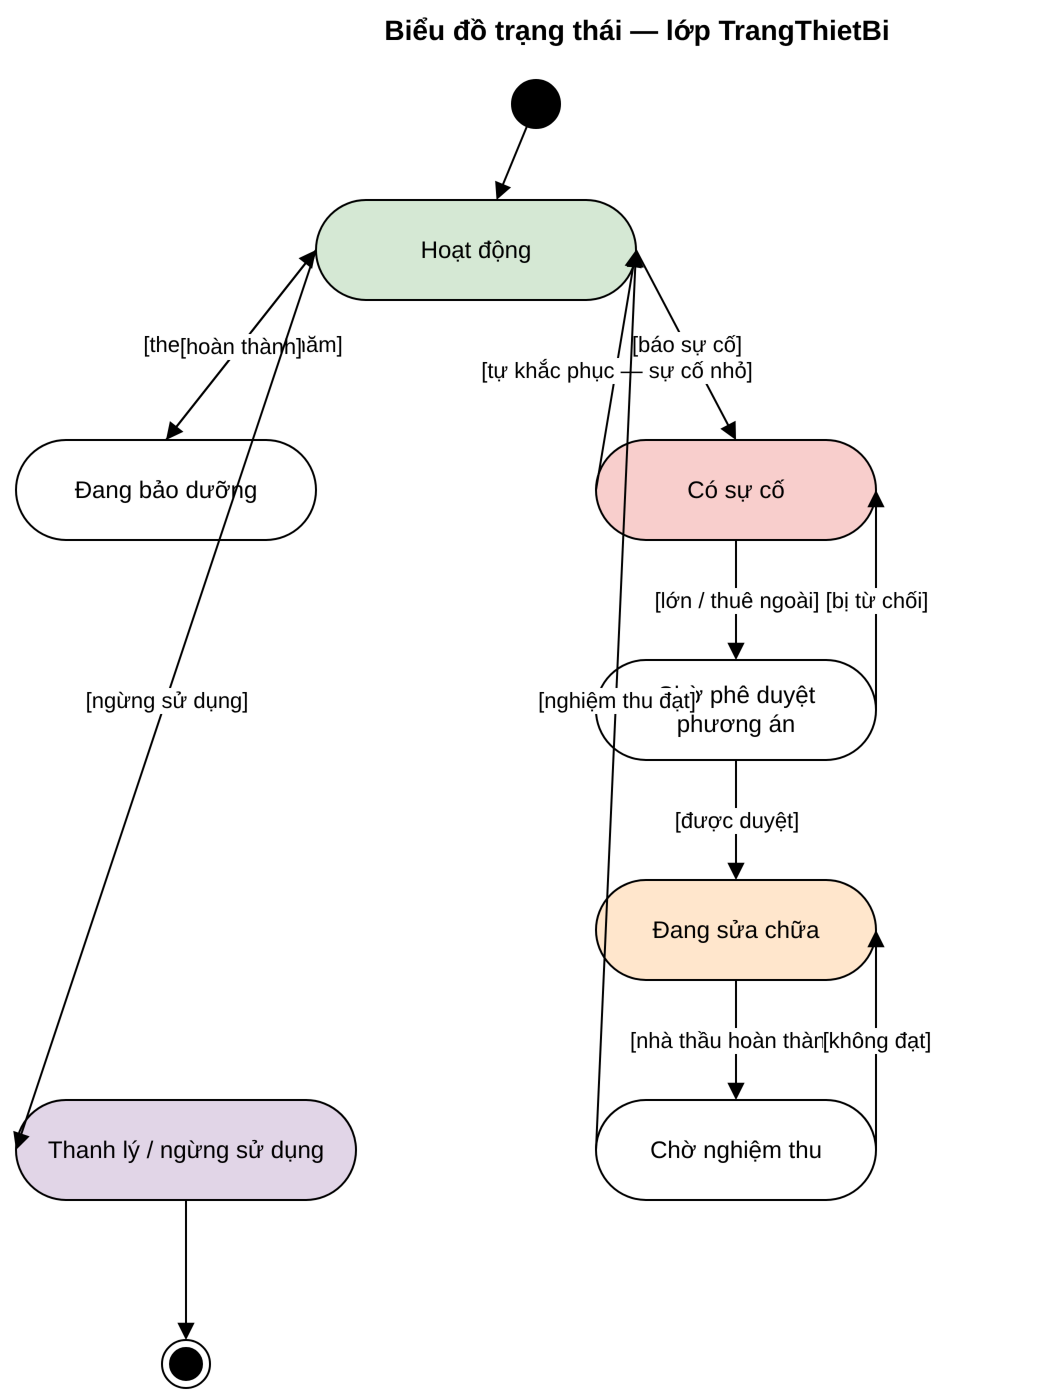
\includegraphics[width=0.72\textwidth]{figures/state-equipment.png}}{\fbox{\parbox{0.9\textwidth}{\centering Sơ đồ trạng thái TrangThietBi (file \texttt{docs/diagrams/05-state.drawio}, trang 1)}}}
\caption{Sơ đồ trạng thái của lớp TrangThietBi}
\label{fig:state-equip}
\end{figure}

\begin{table}[h]
\centering
\caption{Bảng chuyển tiếp trạng thái của TrangThietBi}
\label{tab:state-equip}
\begin{tabular}{P{2.6cm}P{3.4cm}P{9.2cm}}
\toprule
\textbf{Từ} & \textbf{Đến} & \textbf{Sự kiện / điều kiện} \\
\midrule
(bắt đầu) & Hoạt động & Thiết bị được đưa vào danh mục \\
Hoạt động & Đang bảo dưỡng & Theo kế hoạch năm đã duyệt (hạng mục bắt đầu) \\
Đang bảo dưỡng & Hoạt động & Hoàn thành hạng mục — tự ghi hồ sơ BM/02 \\
Hoạt động & Có sự cố & Đơn vị báo sự cố / nguy cơ \\
Có sự cố & Hoạt động & [sự cố nhỏ] Đơn vị tự khắc phục + cập nhật hồ sơ \\
Có sự cố & Chờ phê duyệt & [lớn / thuê ngoài] Chờ lập và duyệt phương án \\
Chờ phê duyệt & Đang sửa chữa & Lãnh đạo Cục phê duyệt phương án \\
Chờ phê duyệt & Có sự cố & Phương án bị từ chối \\
Đang sửa chữa & Chờ nghiệm thu & Nhà thầu/nội bộ báo hoàn thành \\
Chờ nghiệm thu & Hoạt động & Nghiệm thu đạt — đủ chữ ký biên bản BM/04 \\
Chờ nghiệm thu & Đang sửa chữa & Nghiệm thu không đạt \\
Hoạt động & Thanh lý / ngừng sử dụng & Quyết định ngừng sử dụng (hồ sơ BM/02 lưu đến khi máy không sử dụng) \\
Thanh lý & (kết thúc) & Tháo khỏi danh mục hoạt động \\
\bottomrule
\end{tabular}
\end{table}

\subsection{Vòng đời SuCo}

\begin{figure}[h]
\centering
\IfFileExists{figures/state-incident.png}{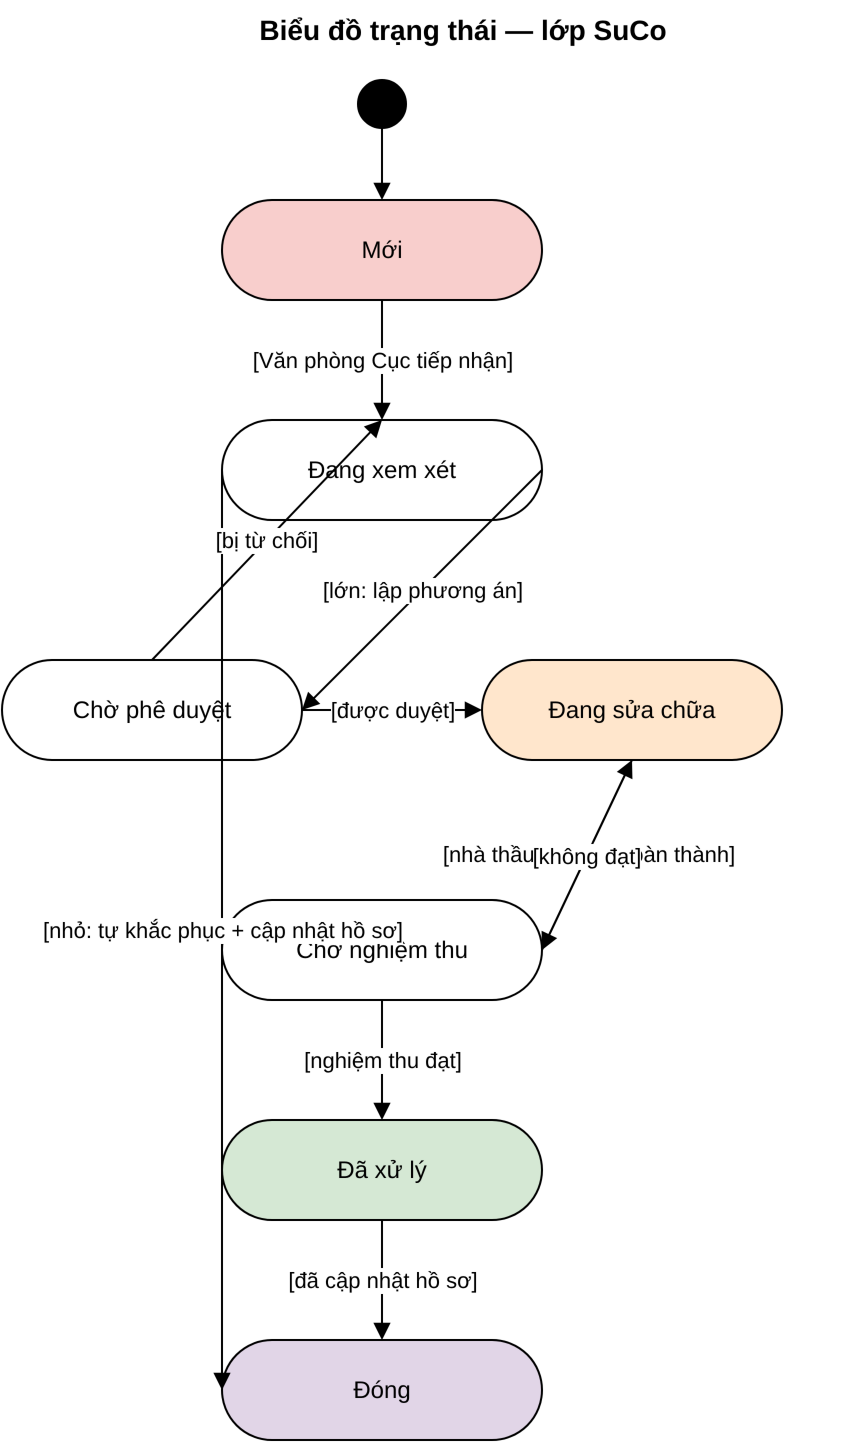
\includegraphics[width=0.72\textwidth]{figures/state-incident.png}}{\fbox{\parbox{0.9\textwidth}{\centering Sơ đồ trạng thái SuCo (file \texttt{docs/diagrams/05-state.drawio}, trang 2)}}}
\caption{Sơ đồ trạng thái của lớp SuCo}
\label{fig:state-incident}
\end{figure}

Điểm đáng chú ý của Hình~\ref{fig:state-incident}: từ ``Đang xem xét'' có hai đường rời đi phản ánh đúng quy trình — \textbf{[nhỏ: tự khắc phục + cập nhật hồ sơ]} đi thẳng tới ``Đóng'' (bỏ qua phê duyệt), còn \textbf{[lớn: lập phương án]} đi qua ``Chờ phê duyệt''. Trạng thái ``Chờ phê duyệt'' khi bị từ chối quay về ``Đang xem xét'' (lập lại phương án), không mất dữ liệu.

\section{Kết luận chương}

Ba loại sơ đồ hành vi (trình tự, trạng thái) được xây dựng cho hai luồng nghiệp vụ cốt lõi và hai lớp then chốt, bảo đảm: (i) nhất quán với sơ đồ use case (Chương 3) và sơ đồ lớp (Chương 4); (ii) đúng ngữ nghĩa quy trình gốc — đặc biệt nhánh sự cố nhỏ không qua phê duyệt; (iii) đủ cơ sở cho thiết kế state machine trong mã nguồn (Chương 6).
